%=====================================================================
\section{Data, Measurement and Descriptive Evidence}\label{sec:eda}
%=====================================================================

The results reported in the preceding introduction rest on a sizeable panel, and it is worth
making the measurement conventions explicit before adding further empirical analysis. This
section documents the source file, the transformation from raw judge scores to weekly shares,
the notation used throughout, and the descriptive structure of both the raw and reconstructed
data. Every number below is computed directly from the distributed CSV files.

\subsection{Source Data and Panel Construction}\label{sec:eda_source}

The official data file contains \textbf{421 contestants} across \textbf{34 seasons}. Each row
records the celebrity, the professional partner, industry, home state/country, age during the
season, the final result and placement, and up to eleven weeks of scores from up to four judges.
After coercing non-numeric entries (``N/A'' and blanks) to missing values, we obtain
\textbf{18{,}524} usable judge-score entries with mean $5.235$, standard deviation $3.942$,
and range $0$ to $13.333$; values above $10$ arise in weeks where multiple dances are averaged,
as the data description specifies. Celebrity ages run from $14$ to $82$ with mean $38.79$.
The industry composition is dominated by actors ($128$), athletes ($95$), television
personalities ($67$) and singers ($61$), with models ($17$) and a long tail of smaller categories.

The reconstruction panel built from these data contains \textbf{2{,}777 couple--weeks},
organised into \textbf{335} competition weeks, of which \textbf{266} contain at least one
elimination. There are \textbf{308} eliminated couple--week records because some weeks eliminated
two or even three couples (the recorded maximum of $n_{\rm exit}$ is $3$). Weeks in which no
couple left are retained for the uncertainty analysis but are excluded from elimination-hit
statistics. The longest season spans $11$ competition weeks; the mean field size is $8.29$
couples per week, ranging from $2$ to $16$.

\begin{table}[H]
\centering
\caption{Notation used in the extended analysis.}
\label{tab:notation}
\begin{tabular}{ll}
\toprule
Symbol & Meaning \\
\midrule
$S_{sw}$              & set of couples surviving in week $w$ of season $s$; $n_{sw}=|S_{sw}|$ \\
$q^J_{i,sw}$          & judge share: couple $i$'s weekly judge total divided by $\sum_{j\in S_{sw}}J_{j,sw}$ \\
$r^J_{i,sw}$          & ordinal judge rank within the week ($1$ = best) \\
$\hat q^F_{i,sw}$     & posterior median of the reconstructed fan share (Model~1) \\
$\tilde q^F_{i,sw}$   & within-week renormalisation $\hat q^F_i/\sum_j\hat q^F_j$ \\
$\sigma^F_{i,sw}$     & posterior standard deviation of the fan share \\
$\Delta_{i,sw}$       & width of the $90\%$ credible interval, $q^F_{95}-q^F_{5}$ \\
$\Delta^{\rm rel}$    & field-size-normalised width, $n_{sw}\,\Delta$ \\
$r^F_{i,sw}$          & ordinal rank of the reconstructed fan share \\
$w$                   & counterfactual fusion weight placed on the judge channel \\
$\hat R$, ESS         & split-$\hat R$ convergence diagnostic and effective sample size \\
\bottomrule
\end{tabular}
\end{table}

Two conventions matter for interpreting the numbers that follow. First, $\hat q^F$ is the
\emph{raw} posterior median on the feasible polytope; its within-week sum is generally below one
because the sampler does not force a unit simplex. For counterfactual score comparisons, where
the judge and fan channels must live on the same scale, we instead use $\tilde q^F$. Second,
every within-week quantity is computed only over couples still in the competition; including
already-eliminated couples (whose judge scores are recorded as zero) would bias all shares
toward zero and is deliberately avoided.

\subsection{Descriptive Structure of the Raw and Reconstructed Data}

Figure~\ref{fig:paneloverview} summarises the panel. Panel~(a) shows that season length is far
from constant: early seasons contribute few couple--weeks while the middle and late seasons
contribute $80$--$120$ each. This matters because any pooled statistic is implicitly weighted
toward the longer seasons, which is why we report both pooled and season-stratified quantities
in Section~\ref{sec:empirical}. Panel~(b) shows the field-size distribution, with a mean of
$8.29$ couples and a long right tail up to $16$. Panel~(c) confirms the expected score
inflation: weekly judge totals rise as weaker dancers are removed and the surviving couples
master more demanding routines. Panel~(d) shows the age distribution of the raw contestants,
which is right-skewed with a mode in the late twenties.

\begin{figure}[H]
\centering
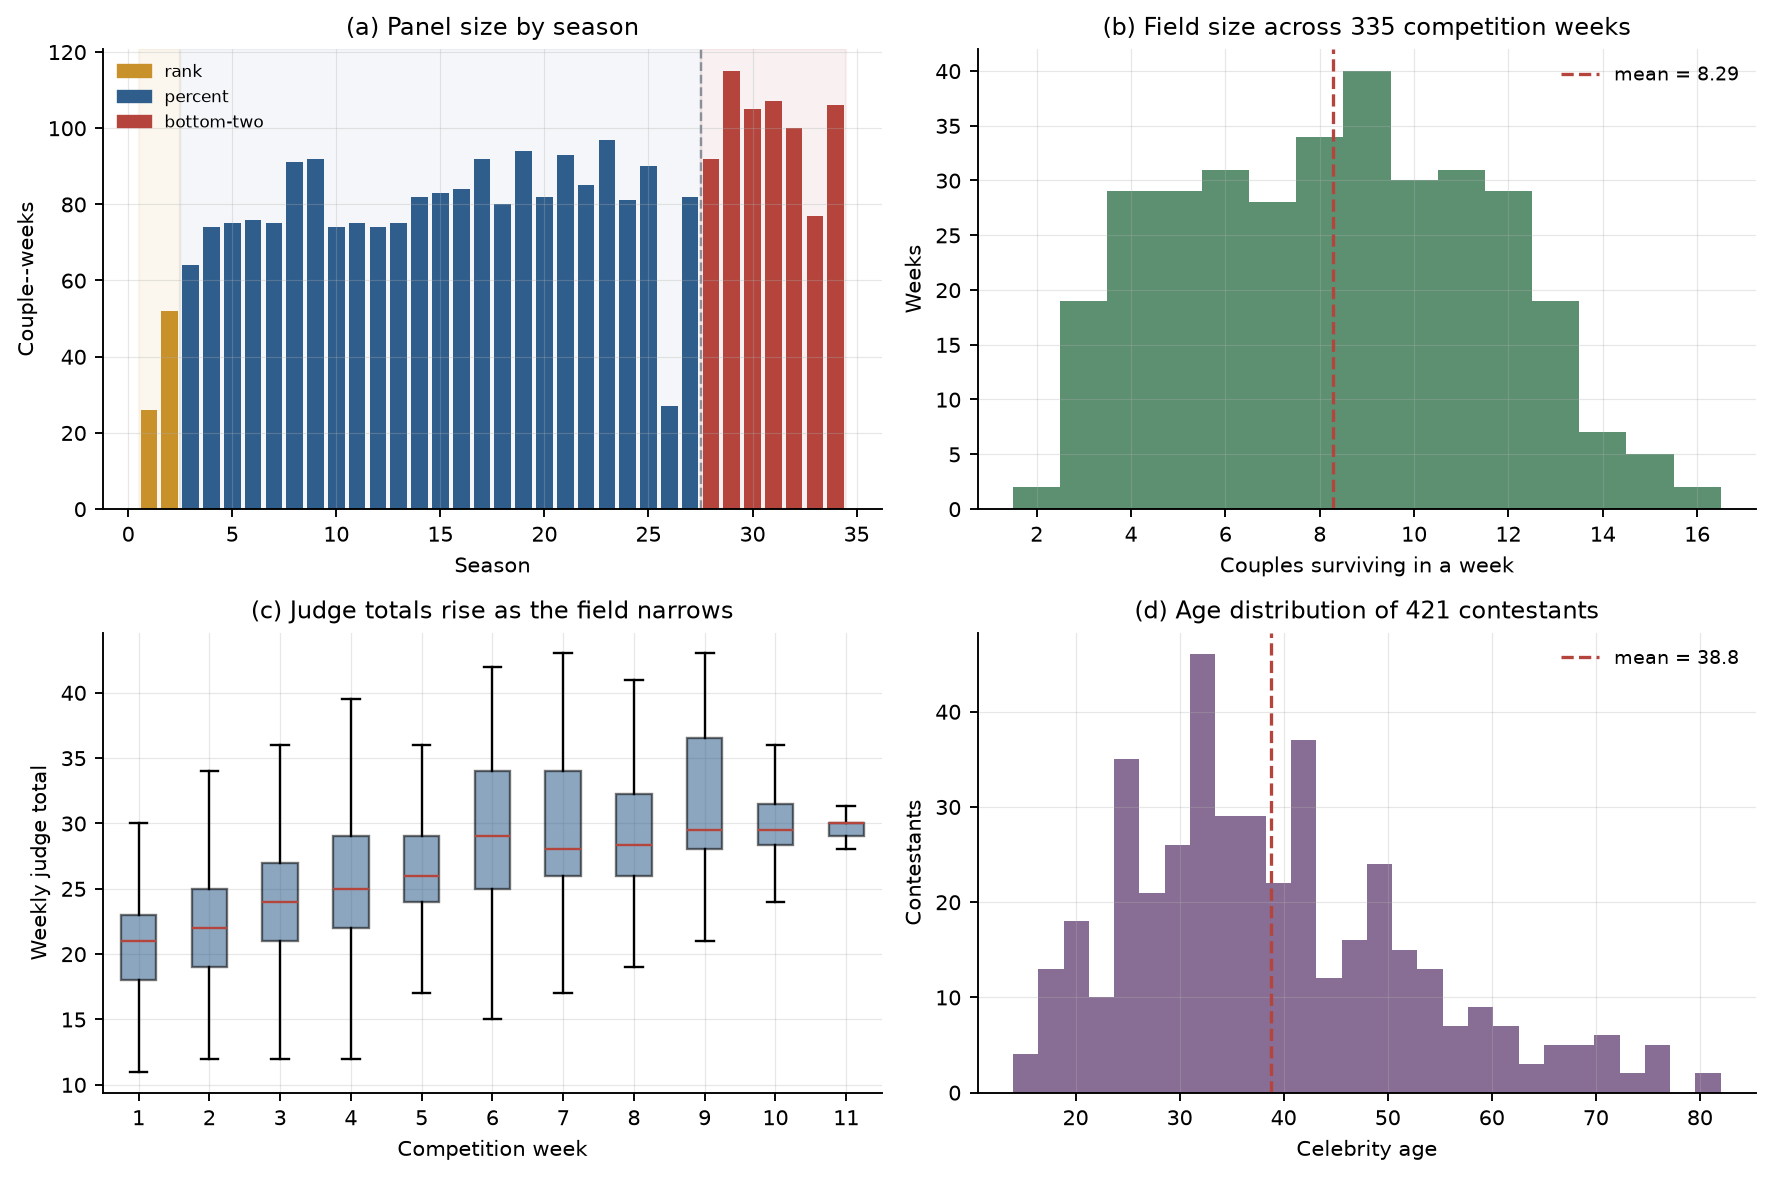
\includegraphics[width=0.94\textwidth]{figures_ext/fig01_panel_overview.png}
\caption{Panel construction and raw-data descriptives. (a) Couple--weeks per season, coloured
by fusion regime (gold = rank, blue = percent, red = bottom-two). (b) Distribution of weekly
field size over 335 competition weeks. (c) Distribution of weekly judge totals by competition
week (boxes show the interquartile range; outliers suppressed). (d) Age distribution of the
421 contestants in the official data file.}
\label{fig:paneloverview}
\end{figure}

Figure~\ref{fig:rawscores} turns to the raw judge scores themselves. Panel~(a) shows a
right-skewed distribution of $18{,}524$ individual scores with mean $5.235$; the mass near zero
comes from weeks where a couple had already been eliminated but the score columns were populated.
Panel~(b) plots the week-by-week mean and standard deviation, making the seasonal score
inflation explicit: the average score roughly doubles from the first week to the final week.
Because $q^J$ is a \emph{within-week} share, this common inflation is differenced out and does
not contaminate the judge channel. Panels~(c) and~(d) describe the casting composition and the
split between finalists and eliminated contestants.

\begin{figure}[H]
\centering
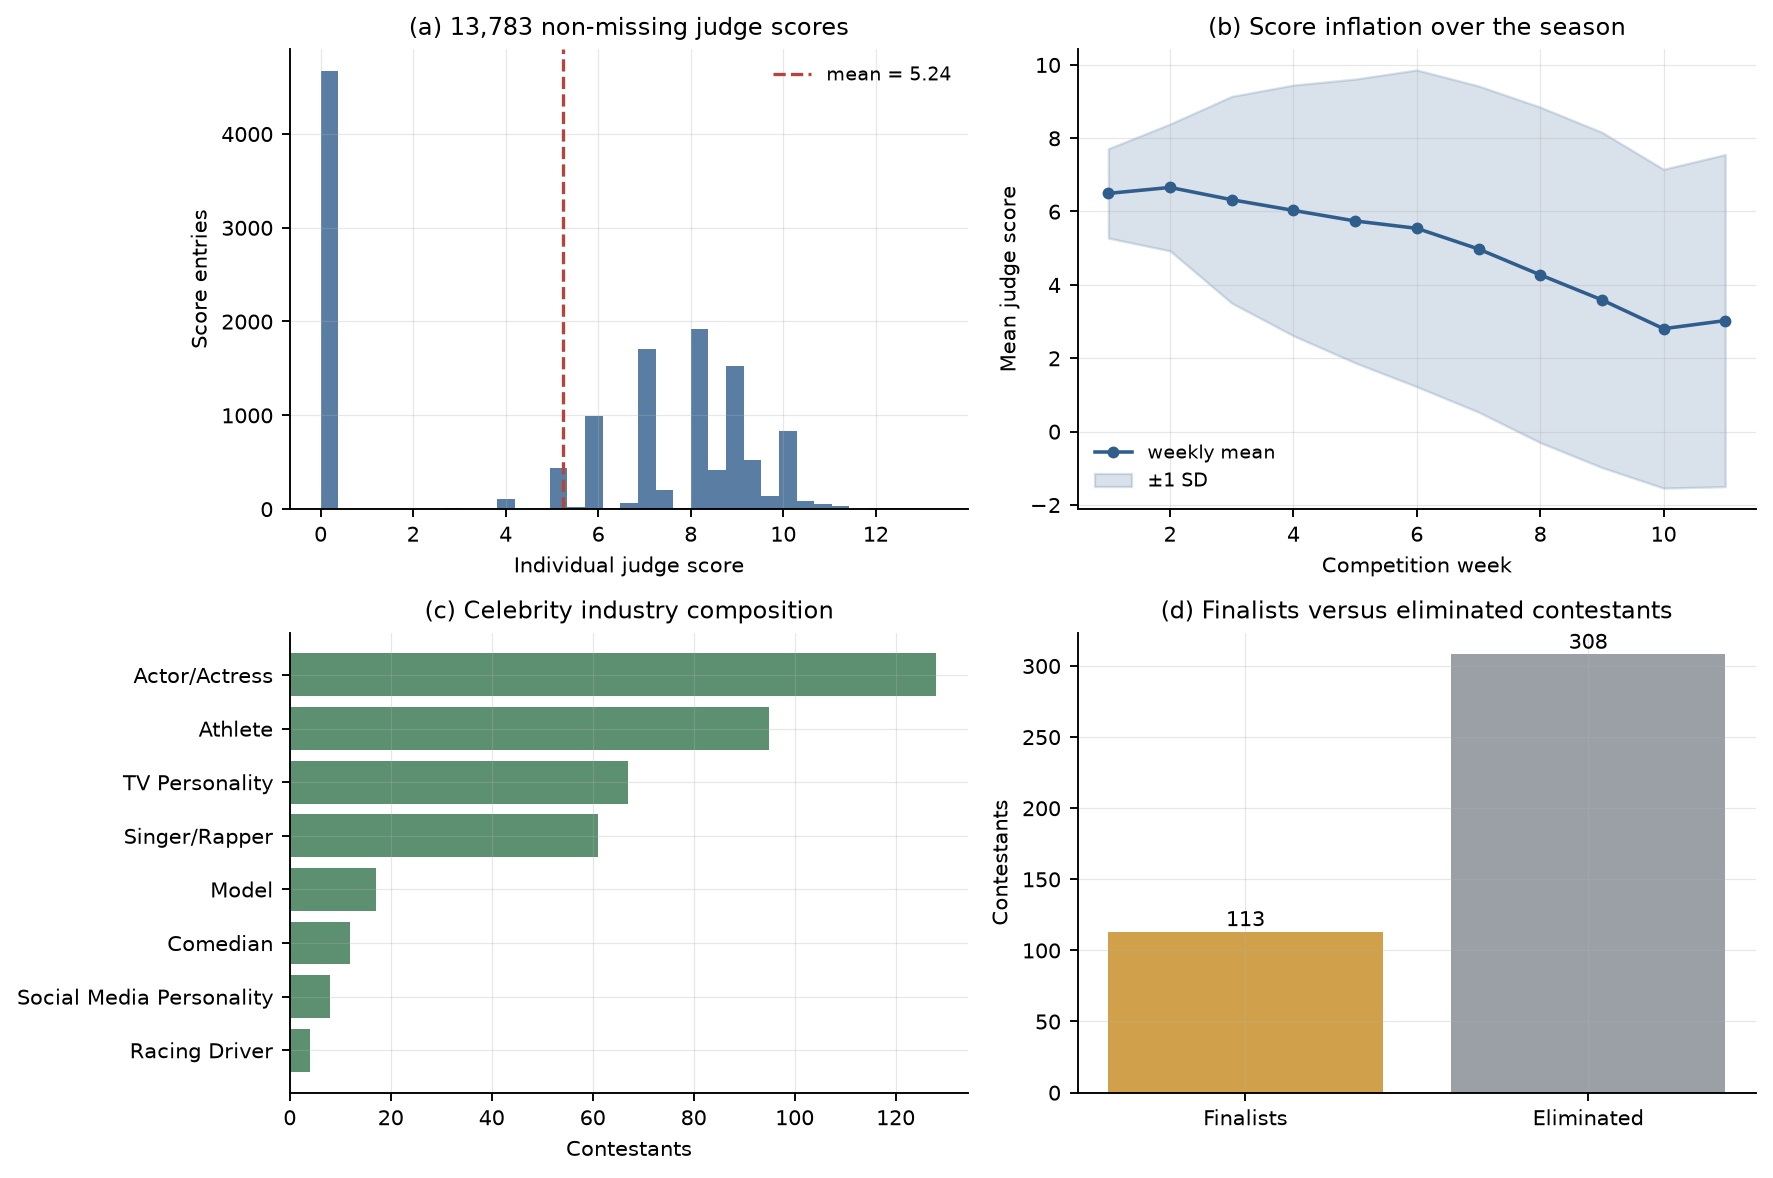
\includegraphics[width=0.94\textwidth]{figures_ext/fig02_raw_judge_scores.png}
\caption{Descriptive statistics of the official judge-score columns. (a) Histogram of all
non-missing individual judge scores. (b) Mean $\pm$ one standard deviation of the weekly
averaged judge score by competition week. (c) The eight largest industry categories.
(d) Contestants placing as finalists versus those eliminated during the season.}
\label{fig:rawscores}
\end{figure}

\subsection{Correlation Definitions and a Caution on Terminology}

Two headline correlations appear throughout the paper and are easy to misread, so we define
them precisely. The value $\mathbf{0.832}$ is the \emph{Pearson} product-moment correlation
between $q^J$ and the raw posterior median $\hat q^F$ over all $2{,}777$ couple--weeks; the
corresponding Spearman coefficient is $0.677$. The value $\mathbf{0.153}$ is the \emph{Pearson}
correlation between the two ordinal rank vectors $r^J$ and $r^F$ (its Spearman counterpart is
$0.079$). Neither is a Spearman rank correlation in the classical sense, and we retain the
original wording for consistency with the main text while making the definitions explicit here.
The counterfactual analysis uses $\tilde q^F$, for which the Pearson correlation with $q^J$ is
$0.807$ and the Spearman correlation $0.660$. Table~\ref{tab:corrdefs} collects all four
definitions; the difference between $0.832$ and $0.807$ is purely the renormalisation, not a
change in the underlying estimates.

% AUTO-GENERATED table — values computed by analyze_extended.py
\begin{table}[H]
\centering
\caption{Correlation definitions used in this paper. The headline $0.832$ is the Pearson correlation of $q^J$ with the unnormalised posterior median $\hat q^F$; the counterfactual replay instead uses the within-week renormalised share $\tilde q^F=\hat q^F/\sum_i\hat q^F_i$, so its Pearson correlation with $q^J$ is slightly lower. The headline $0.153$ is the Pearson correlation of the two rank vectors $r^J,r^F$, not a Spearman coefficient.}
\label{tab:corrdefs}
\begin{tabular}{lrr}
\toprule
Pair & Pearson & Spearman \\ 
\midrule
$q^J$ vs.\ $\hat q^F$ (headline) & 0.832 & 0.676 \\ 
$q^J$ vs.\ $\tilde q^F$ (replay) & 0.807 & 0.660 \\ 
$q^J$ vs.\ percent-combined & 0.941 & 0.883 \\ 
$r^J$ vs.\ $r^F$ (headline rank) & 0.153 & 0.079 \\ 
\bottomrule
\end{tabular}
\end{table}


The gap between the level correlation ($0.832$) and the rank-vector correlation ($0.153$) is
the single most important descriptive fact in the data: judges and fans agree about \emph{how
much} support a couple has in broad terms, but disagree substantially about the fine ordering
inside the field. Since rank fusion consumes only the fine ordering while percent fusion consumes
the magnitudes, this discrepancy is precisely the mechanism that makes the rule choice matter.
Section~\ref{sec:empirical} quantifies it directly.

%=====================================================================
